%Este trabalho está licenciado sob a Licença Creative Commons Atribuição-CompartilhaIgual 4.0 Internacional. Para ver uma cópia desta licença, visite https://creativecommons.org/licenses/by-sa/4.0/ ou envie uma carta para Creative Commons, PO Box 1866, Mountain View, CA 94042, USA.


\chapter{Introdução às funções}

Quando estudamos fenômenos, buscamos estabelecer relações entre informações. Por exemplo, a área de um quadrado depende da medida do seu lado.

\begin{obs}
  Dados dois conjuntos $A$ e $B$ não vazios, uma \textbf{função} de $A$ em $B$ (ou \textbf{aplicação}) é uma regra (expressão) que diz como associar \emph{cada} elemento $x \in A$ a um \emph{único} $y \in B$.
\end{obs}

Usamos normalmente a seguinte notação:
\begin{equation*}
f: A \rightarrow B
\end{equation*}
que se lê: $f$ é uma função de $A$ em $B$.

A função $f$ transforma $x \in A$ em $y \in B$. Denotamos isso da seguinte forma:
\begin{equation*}
f(x) = y .
\end{equation*}

Simplificando as notações podemos representar as duas informações acima da seguinte forma:
\begin{eqnarray*}
 f: A & \rightarrow & B \\
 x & \mapsto & y.
\end{eqnarray*}

 Exemplos de relações que são funções de $A$ em $B$:
 \begin{multicols}{3}
 \begin{center}
 \begin{tikzpicture}[scale=0.50]
 \node (1) at (0,0) {1};%\filldraw(1.east) circle (1pt)
 \node (2) [below of=1] {2};%\filldraw(2.east) circle (1pt)
 \node (3) [below of=2] {3};%\filldraw(3.east) circle (1pt)
 \node[fit=(1) (2) (3),ellipse,draw=red,minimum width=1cm,thick,label=below:\(A\)]{};

 \node (a) at (3,0) {a};%\filldraw($b_1$.west) circle (1pt)
 \node (b) [below of=a] {b};%\filldraw($b_2$.west) circle (1pt)
 \node (c) [below of=b] {c};%\filldraw($b_3$.west) circle (1pt)
 \node[fit=(a) (b) (c),ellipse,draw=green,minimum width=1cm,thick,label=below:\(B\)]{};

 \draw[->, shorten >=.1cm, >=stealth'] (1.east) to (a.west);
 \draw[->, shorten >=.1cm, >=stealth'] (2.east) to (b.west);
 \draw[->, shorten >=.1cm, >=stealth'] (3.east) to (c.west);
\end{tikzpicture} 
\end{center}

\begin{center}
 \begin{tikzpicture}[scale=0.50]
 \node (1) at (0,0) {1};%\filldraw(1.east) circle (1pt)
 \node (2) [below of=1] {2};%\filldraw(2.east) circle (1pt)
 \node (3) [below of=2] {3};%\filldraw(3.east) circle (1pt)
 \node[fit=(1) (2) (3),ellipse,draw=red,minimum width=1cm,thick,label=below:\(A\)]{};

 \node (a) at (3,0) {a};%\filldraw($b_1$.west) circle (1pt)
 \node (b) [below of=a] {b};%\filldraw($b_2$.west) circle (1pt)
 \node (c) [below of=b] {c};%\filldraw($b_3$.west) circle (1pt)
 \node[fit=(a) (b) (c),ellipse,draw=green,minimum width=1cm,thick,label=below:\(B\)]{};

 \draw[->, shorten >=.1cm, >=stealth'] (1.east) to (a.west);
 \draw[->, shorten >=.1cm, >=stealth'] (2.east) to (a.west);
 \draw[->, shorten >=.1cm, >=stealth'] (3.east) to (c.west);
\end{tikzpicture}
\end{center}

\begin{center}
\begin{tikzpicture}[scale=0.50]
 \node (1) at (0,0) {1};%\filldraw(1.east) circle (1pt)
 \node (2) [below of=1] {2};%\filldraw(2.east) circle (1pt)
 \node (3) [below of=2] {3};%\filldraw(3.east) circle (1pt)
 \node[fit=(1) (2) (3),ellipse,draw=red,minimum width=1cm,thick,label=below:\(A\)]{};

 \node (a) at (3,0) {a};%\filldraw($b_1$.west) circle (1pt)
 \node (b) [below of=a] {b};%\filldraw($b_2$.west) circle (1pt)
 \node (c) [below of=b] {c};%\filldraw($b_3$.west) circle (1pt)
 \node[fit=(a) (b) (c),ellipse,draw=green,minimum width=1cm,thick,label=below:\(B\)]{};

 \draw[->, shorten >=.1cm, >=stealth'] (1.east) to (b.west);
 \draw[->, shorten >=.1cm, >=stealth'] (2.east) to (b.west);
 \draw[->, shorten >=.1cm, >=stealth'] (3.east) to (b.west);
\end{tikzpicture}
\end{center}
\end{multicols}

 Exemplos de relações que não são funções de $A$ em $B$:
\begin{multicols}{2}
\begin{center}
\begin{tikzpicture}[scale=0.50]
 \node (1) at (0,0) {1};%\filldraw(1.east) circle (1pt)
 \node (2) [below of=1] {2};%\filldraw(2.east) circle (1pt)
 \node (3) [below of=2] {3};%\filldraw(3.east) circle (1pt)
 \node[fit=(1) (2) (3),ellipse,draw=red,minimum width=1cm,thick,label=below:\(A\)]{};

 \node (a) at (3,0) {a};%\filldraw($b_1$.west) circle (1pt)
 \node (b) [below of=a] {b};%\filldraw($b_2$.west) circle (1pt)
 \node (c) [below of=b] {c};%\filldraw($b_3$.west) circle (1pt)
 \node[fit=(a) (b) (c),ellipse,draw=green,minimum width=1cm,thick,label=below:\(B\)]{};

 \draw[->, shorten >=.1cm, >=stealth'] (1.east) to (a.west);
 \draw[->, shorten >=.1cm, >=stealth'] (1.east) to (b.west);
 \draw[->, shorten >=.1cm, >=stealth'] (2.east) to (b.west);
 \draw[->, shorten >=.1cm, >=stealth'] (3.east) to (c.west);
\end{tikzpicture}
\end{center}

Não é função pois o elemento $1 \in A$ está relacionado aos elementos $a$ e $b$ do conjunto $B$.

\columnbreak

\begin{center}
\begin{tikzpicture}[scale=0.50]
 \node (1) at (0,0) {1};%\filldraw(1.east) circle (1pt)
 \node (2) [below of=1] {2};%\filldraw(2.east) circle (1pt)
 \node (3) [below of=2] {3};%\filldraw(3.east) circle (1pt)
 \node[fit=(1) (2) (3),ellipse,draw=red,minimum width=1cm,thick,label=below:\(A\)]{};

 \node (a) at (3,0) {a};%\filldraw($b_1$.west) circle (1pt)
 \node (b) [below of=a] {b};%\filldraw($b_2$.west) circle (1pt)
 \node (c) [below of=b] {c};%\filldraw($b_3$.west) circle (1pt)
 \node[fit=(a) (b) (c),ellipse,draw=green,minimum width=1cm,thick,label=below:\(B\)]{};

 \draw[->, shorten >=.1cm, >=stealth'] (1.east) to (a.west);
 %\draw[->, shorten >=.1cm, >=stealth'] (2.east) to (b.west);
 \draw[->, shorten >=.1cm, >=stealth'] (3.east) to (c.west);
\end{tikzpicture}
\end{center}
Não é função pois o elemento $2 \in A$ não está relacionado com nenhum elemento do conjunto $B$.

% \begin{tikzpicture}[scale=0.50]
%  \node (1) at (0,0) {1};%\filldraw(1.east) circle (1pt)
%  \node (2) [below of=1] {2};%\filldraw(2.east) circle (1pt)
%  \node (3) [below of=2] {3};%\filldraw(3.east) circle (1pt)
%  \node[fit=(1) (2) (3),ellipse,draw=red,minimum width=1cm,thick,label=below:\(A\)]{};

%  \node (a) at (3,0) {a};%\filldraw($b_1$.west) circle (1pt)
%  \node (b) [below of=a] {b};%\filldraw($b_2$.west) circle (1pt)
%  \node (c) [below of=b] {c};%\filldraw($b_3$.west) circle (1pt)
%  \node[fit=(a) (b) (c),ellipse,draw=green,minimum width=1cm,thick,label=below:\(B\)]{};

%  \draw[->, shorten >=.1cm, >=stealth'] (1.east) to (a.west);
%  \draw[->, shorten >=.1cm, >=stealth'] (1.east) to (b.west);
%  %\draw[->, shorten >=.1cm, >=stealth'] (2.east) to (b.west);
%  \draw[->, shorten >=.1cm, >=stealth'] (3.east) to (c.west);
% \end{tikzpicture}

% Não é função pois o elemento $1 \in A$ está relacionado aos elementos $a$ e $b$ do conjunto $B$ e o elemento $2 \in A$ não está relacionado com nenhum elemento do conjunto $B$
\end{multicols}

Dada uma função $f: A \rightarrow B$, o conjunto $A$ chama-se \textbf{domínio} da função $f$ e o conjunto $B$ chama-se \textbf{contradomínio} da função $f$.  Para cada $x \in A$, o elemento $f(x)= y \in B$ chama-se imagem de $x$ pela função $f$. Assim o conjunto \textbf{imagem} da função $f$ é dado por:
\begin{equation*}
Im(f)= \{ y \in B \mid y = f(x) \text{ para algum } x \in A\} .
\end{equation*}

Uma função de uma variável é dita real se $A\subset \R$ e $B\subset \R$.

%No nosso contexto, o domínio de uma função é um subconjunto dos números reais nos quais faz sentido aplicar a regra da função, e o contradomínio é o conjunto $\mathbb{R}$, ou um subconjunto de $\mathbb{R}$ que contenha o conjunto $Im(f)$.

O \textbf{gráfico} da função é dado por:
\begin{equation*}
Gr(f) = \{ (x, f(x)) \in A \times B \mid x \in A\}.
\end{equation*}

Assim, o gráfico de $f$ é um subconjunto do conjunto de todos os pares ordenados $(x,y)$ de números reais.

\begin{obs}
    As raízes de uma função são os valores $x$ do domínio tal que $f(x)=0$.
\end{obs}

% \begin{exem}
%  Considere os conjuntos $A= \{1, 2, 3\}$ e $B= \{a, b, c, d\}$ e a regra de relação entre estes dois conjuntos dada pelo diagrama abaixo:

%  \begin{figure}[H]
%  \centering
%  \begin{tikzpicture}
%  \node (1) at (0,0) {1};%\filldraw(1.east) circle (1pt)
%  \node (2) [below of=1] {2};%\filldraw(2.east) circle (1pt)
%  \node (3) [below of=2] {3};%\filldraw(3.east) circle (1pt)
%  \node[fit=(1) (2) (3),ellipse,draw=red,minimum width=1cm,thick,label=below:\(A\)]{};

%  \node (a) at (3,0) {a};%\filldraw($b_1$.west) circle (1pt)
%  \node (b) [below of=a] {b};%\filldraw($b_2$.west) circle (1pt)
%  \node (c) [below of=b] {c};%\filldraw($b_3$.west) circle (1pt)
%  \node (d) [below of=c] {d};%\filldraw($b_3$.west) circle (1pt)
%  \node[fit=(a) (b) (c) (d),ellipse,draw=green,minimum width=1cm,thick,label=below:\(B\)]{};

%  \draw[->, shorten >=.1cm, >=stealth'] (1.east) to (b.west);
%  \draw[->, shorten >=.1cm, >=stealth'] (2.east) to (c.west);
%  \draw[->, shorten >=.1cm, >=stealth'] (3.east) to (a.west);
% \end{tikzpicture}
% \end{figure}

% Note que esta regra define uma função $f: A \rightarrow B$, cujo domínio é $Dom(f) = A$, contra-domínio é $CDom(f) = B$, e a imagem é $Im(f)= \{a, b, c\}$, observe que $Im(f) \subset CDom(f)$. Pela definição, temos que o gráfico da $f$ será o conjunto
% \[
% Gr(f)= \{(1, b); (2, c); (3, a)\}
% \]
% que pode ser representado geometricamente como feito na figura abaixo:

% \begin{figure}[H]
%  \centering
%     \fbox{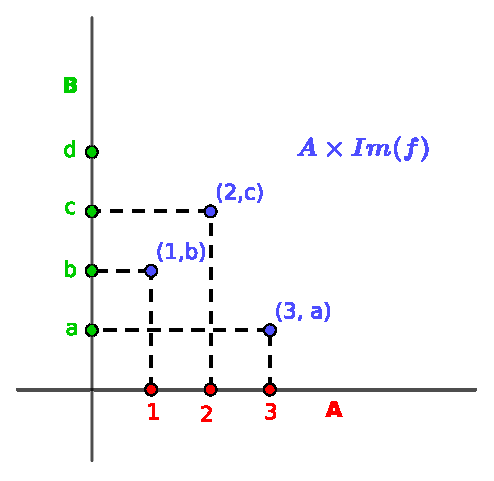
\includegraphics[width=5cm]{./cap_funcao/figs/Grf}}
%     \caption{Gráfico da função $f$}
%   \end{figure}

% \end{exem}


\section{Determinar o maior domínio de uma função real}

Toda função tem que ser composta por domínio, contra-domínio e da expressão da relação. No entanto, é comum uma função real ser apresentada apenas pela expressão da função, sem fazer menção ao seu domínio e contra-domínio. No caso de funções reais, podemos sempre assumir que seu contra-domínio é o conjunto dos números reais $\R$. Porém, o domínio nem sem é todo o conjunto e, assim, precisamos determinar o maior domínio $A\subset \R$ da função que satisfaça a lei de correspondência definida.

\begin{exem}\hfill
    \begin{enumerate}
        \item Para $f(x)=-x$, o maior domínio é $\R$;
        \item Para $f(x)=\frac{1}{x}$, o maior domínio é $\R^{*}$, pois não é possível dividir por zero;
        \item Para $f(x)=\sqrt{x}$, o maior domínio é $\R_{+}$, pois não existe raiz quadrada de número negativo.
    \end{enumerate}
\end{exem}

Note que algumas operações fornecem restrições no domínio. Por enquanto, podemos destacar duas delas:
\begin{itemize}
    \item Divisão por zero: se $f(x)=\dfrac{g(x)}{h(x)}$ então $h(x)\neq 0$;
    \item Raiz de índice par: se $f(x)=\sqrt[par]{g(x)}$ então $g(x)\geq 0$.
\end{itemize}

É possível combinar os dois casos anteriores: se $f(x)=\dfrac{g(x)}{\sqrt[par]{h(x)}}$ então $h(x)> 0$.

\begin{exem}
    Determine o maior domínio da função real $f(x)=\dfrac{1}{x+1}+\sqrt{-x}$.

    A fração fornece a restrição: $x+1= 0$, ou seja, devemos ter $x\neq -1$.

    A raiz quadrada diz que $-x\geq 0$, ou seja, $x\leq 0$.

    Portanto, o maior domínio de $f$ é $A=(-\infty,-1)\cup(-1,0]$.
\end{exem}

% \section{Operações com funções}
% Dadas as funções $f: A \rightarrow \R$, $g: B \rightarrow \R$, se $A \cap B \neq \emptyset$, então $\forall x \in A \cap B$, definimos as seguintes operações entre estas funções:
% \begin{equation*}
% (f + g)(x)= f(x) + g(x); 
% \end{equation*}
% \begin{equation*}
% (f - g)(x)= f(x) - g(x); 
% \end{equation*}
% \begin{equation*}
% (f \cdot g)(x)= f(x) \cdot g(x); 
% \end{equation*}
% \begin{equation*}
%  \left( \frac{f}{g} \right) (x)= \frac{f(x)}{g(x)} ;
% \end{equation*}
% \begin{equation*}
% (k \cdot f)(x)= k \cdot f(x), \text{ para } k \text{ constante} ,
% \end{equation*}

% note que:
% \begin{equation*}
% dom(f+g)= dom(f-g)= dom(f \cdot g)= dom(k \cdot f)= A \cap B ,
% \end{equation*}
% \begin{equation*}
%  dom\left( \frac{f}{g} \right)= \{x \in A \cap B \mid g(x) \neq 0\}. 
% \end{equation*}

\section{Função constante}

A função contante é a função que associa todos os elementos do domínio a um único elemento do contradomínio. Ou seja, dado $a \in \R$ fixo, a função $f$:
\begin{eqnarray*}
 f: \R & \rightarrow & \R \\
 x & \mapsto & a,
\end{eqnarray*}
é uma função constante.

Por exemplo, a função $f:\R\to\R$ tal que $f(x)=2$ é uma função constante. Para construir o gráfico desta função começamos encontrando alguns pontos $(x, y)= (x, f(x))$ do gráfico, o que pode ser feito através da seguinte tabela:

 \begin{table}[H]
 \centering
 \begin{tabular}{|c|c|c|} \hline
 \rowcolor{gray}
  x & f(x) & (x, y)  \\\hline
  -1 & f(-1)= 2 & (-1, 2) \\\hline
   0 & f(0)= 2 & (0, 2)  \\\hline
   1 & f(1)= 2 & (1, 2) \\\hline
 \end{tabular}
\end{table}

Após encontrar os pontos basta marcar os mesmo o plano cartesiano e traçar a curva que liga estes pontos com isso objetos o gráfico da função. Neste caso o gráfico é:
\begin{figure}[H]
 \centering
    \fbox{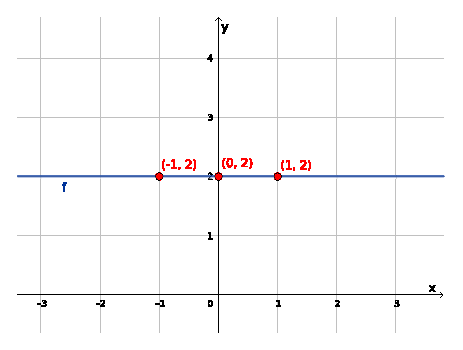
\includegraphics[width=7cm]{./cap_funcao/figs/f(x)=2}}
    \caption{Gráfico da função $f(x)=2$}
  \end{figure}

\section{Função identidade}

A função $Id$:
\begin{eqnarray*}
 Id: \R & \rightarrow & \R \\
 x & \mapsto & x \ ,
\end{eqnarray*}
é chamada \textit{função identidade real}.

Para encontrar alguns pontos $(x, f(x))$ do gráfico desta função, construímos a seguinte tabela:

 \begin{table}[H]
 \centering
 \begin{tabular}{|c|c|c|} \hline
 \rowcolor{gray}
  x & f(x) & (x, y)  \\\hline
  -1 & f(-1)= -1 & (-1, -1) \\\hline
   0 & f(0)= 0 & (0, 0)  \\\hline
   1 & f(1)= 1 & (1, 1) \\\hline
 \end{tabular}
\end{table}

Logo o gráfico da função $Id$ é:
\begin{figure}[H]
 \centering
    \fbox{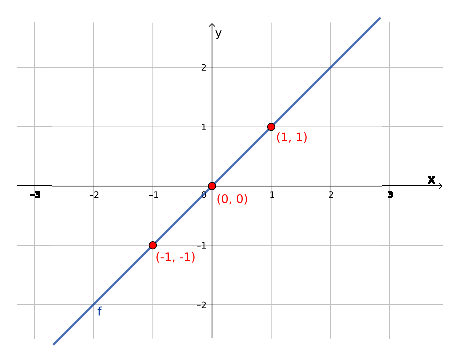
\includegraphics[width=7cm]{./cap_funcao/figs/Id(x)=x}}
    \caption{Gráfico da função $Id(x)=x$}
  \end{figure}


\section{Funções do 1º grau}
 As funções do 1º grau, ou funções afim são funções $f: \R \rightarrow \R$ dadas por:
\begin{equation*}
f(x)= ax + b \ , 
\end{equation*}
para certos $a, b \in \R$ com $a \neq 0$. Note que um caso particular e já conhecido de função de 1º grau é a função identidade, $f(x)= x$, a qual possui $a=1$ e $b=0$.

 Vejamos mais alguns exemplos de funções de 1º grau.

\begin{exem}
 Consideremos as funções $f, g: \R \to \R$ dadas por:
 \begin{enumerate}[a)]
  \item $f(x)= x+2$
  \item $g(x)= x-1$
 \end{enumerate}


 \begin{figure}[H]
   \fbox{\subfigure[$f(x)= x+2$]{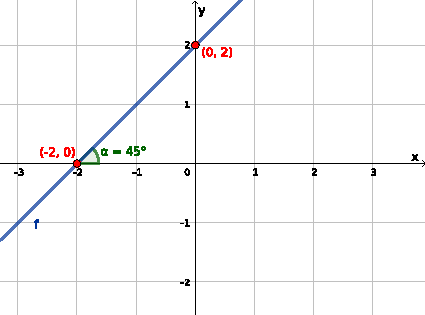
\includegraphics[width=7cm,height=6cm]{./cap_funcao/figs/f(x)=x+2}}}
   \fbox{\subfigure[$g(x)= x-1$]{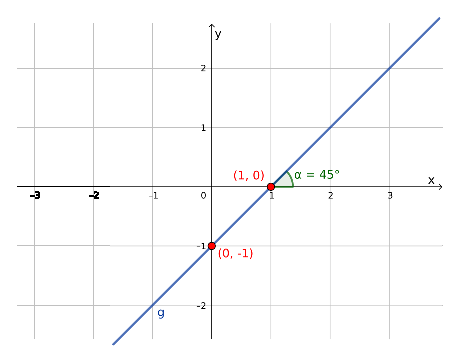
\includegraphics[width=7cm,height=6cm]{./cap_funcao/figs/f(x)=x-1}}}
  \end{figure}
  Note que o que muda na definição destas funções é apenas o coeficiente $b$. Fazendo uma análise comparativa dos gráficos destas funções notamos que os ângulos que as retas formam com o eixo $x$ é o mesmo, portanto as retas são paralelas, porém o ponto de interseção das retas com o eixo $y$, que são os pontos $(0, f(0))$, $(0, g(0))$ muda, ou seja, $f(0) \neq g(0)$. De fato:
\begin{equation*}
f(0)= 0 + 2= 2
\end{equation*}
\begin{equation*}
g(0)= 0 -1 = -1 \ .
\end{equation*}
\end{exem}
  
  No caso geral em que $f(x)=ax+b$, teremos que $f(0)=a0 + b= b$, portanto o gráfico de $f$ irá intersectar o eixo $y$ no ponto $(0,b)$. O coeficiente $b$ é chamado de \textbf{coeficiente linear} da reta/função linear.

\begin{exem}
  Consideremos as funções $f, g: \R \to \R$ dadas por:
 \begin{enumerate}[a)]
  \item $f(x)= 2x$
  \item $g(x)= -2x$
 \end{enumerate}

 \begin{figure}[H]
   \fbox{\subfigure[$f(x)= 2x$]{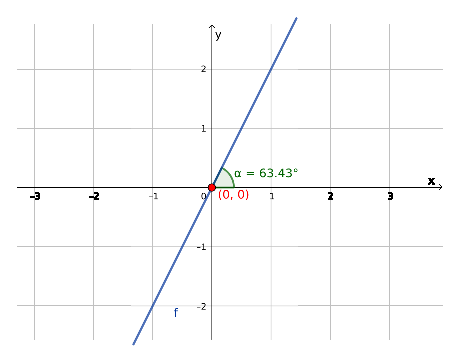
\includegraphics[width=7cm,height=6cm]{./cap_funcao/figs/f(x)=2x}}}
   \fbox{\subfigure[$g(x)= -2x$]{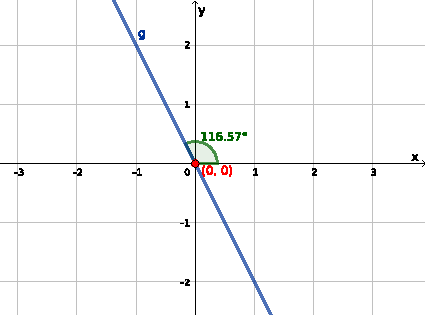
\includegraphics[width=7cm,height=6cm]{./cap_funcao/figs/g(x)=-2x}}}
  \end{figure}
    
  Neste exemplos estamos mudando apenas o coeficiente $a$ das funções, o que está alterando o ângulo que as retas formam com o eixo $x$, ou seja a inclinação das retas em relação ao eixo $x$. Já o ponto de interseção das retas com o eixo $y$ é o mesmo pois $f(0)= g(0)= 0$.
  \end{exem}
  
  O coeficiente $a$ é chamado de \textbf{coeficiente angular} da reta/função linear.

\begin{obs}
 O gráfico de uma função linear $f: \R \to \R$ dada por:
\begin{equation*}
f(x) = ax + b
\end{equation*}
 é uma reta com coeficiente angular $a$ e cuja interseção com o eixo $y$ ocorre no ponto $(0, b)$.
\end{obs}

 Frequentemente a equação da reta é dada pela equação $y=mx+n$, que nada mais é do que uma função de 1º grau, basta considerar $y=f(x)$ o que fazemos no contexto de funções para trabalhar com o gráfico da função.

 \subsection{Coeficiente angular da reta}

  Dados dois pontos $P_0=(x_0, y_0)$, $P_1=(x_1, y_1)$, com $x_0 \neq x_1$, como na figura:

 \begin{figure}[H]
 \centering
    \fbox{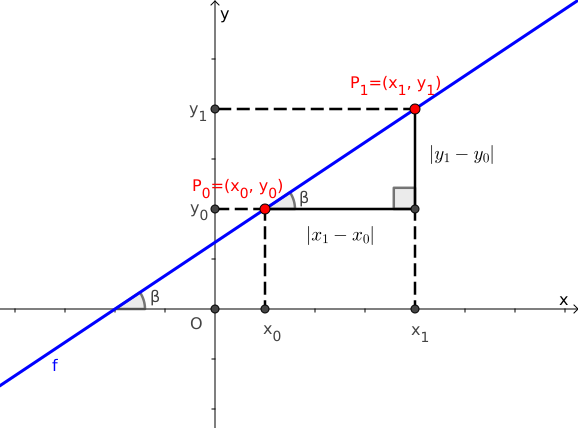
\includegraphics[width=8cm]{./cap_funcao/figs/coefangular}}
    \caption{Coeficiente angular da reta}
  \end{figure}

  O coeficiente angular da reta que passa por estes dois pontos é dado por:
\begin{equation*}
a= \frac{y_1 - y_0}{x_1 - x_0} \ \ \ \text{ ou } \ \ \ a= \frac{y_0 - y_1}{x_0 - x_1} \ .
\end{equation*}

  De fato, dados dois pontos $P_0=(x_0, y_0)$, $P_1=(x_1, y_1)$, com $x_0 \neq x_1$, podemos encontrar a função $f(x)= ax+b$, cujo gráfico passa por estes dois pontos lembrando que ambos devem satisfazer a equação da função assim obtemos:
  \[ \begin{cases}
   y_0= ax_0 + b \\
   y_1= ax_1 + b
  \end{cases} \]
  logo $y_0 - ax_0= b$, substituindo na segunda equação decorre que:
\begin{equation*}
y_1= ax_1 + y_0 - ax_0 \Rightarrow y_1 - y_0= a(x_1 - x_0) \Rightarrow a= \frac{y_1 - y_0}{x_1 - x_0} \ . 
\end{equation*}

  Este sistema linear sempre pode ser usado para encontrar a regra da função linear que passa por dois pontos dados.


  \begin{exem}
  Vamos determinar o coeficiente angular da reta que passa pelos pontos:
   \begin{enumerate}[a)]
    \item $P_0=(0,2)$ e $P_1=(-2,0)$
\begin{equation*}
a= \frac{y_1 - y_0}{x_1 - x_0}= \frac{0 - 2}{-2 - 0}= \frac{-2}{-2}= 1
\end{equation*}
    \item $P_0=(1,2)$ e $P_1=(-1,-2)$
\begin{equation*}
a= \frac{y_1 - y_0}{x_1 - x_0}= \frac{-2 - 2}{-1 - 1}= \frac{-4}{-2}= 2
\end{equation*}
   \end{enumerate}

  \end{exem}

  Quando dados dois pontos $P_0=(x_0, y_0)$, $P_1=(x_1, y_1)$, com $x_0 = x_1$, temos uma reta vertical, cuja equação é $x= a$ para algum $a \in \R$, que não é o gráfico de uma função, por isso não iremos detalhar este caso.

  Dadas duas funções lineares $f(x)=a_1 x + b_1$ e $g(x)= a_2 x + b_2$, tais que $f(x) \neq g(x)$, a partir da análise de seus coeficientes angulares podemos conhecer a posição relativa de seus gráficos. Nesta situação temos dois casos especiais:
  \begin{itemize}
  \item Se $a_1= a_2$ então os gráficos de $f$ e $g$ são retas \textbf{paralelas};
  \item Se $a_1 \cdot a_2= -1$ então os gráficos de $f$ e $g$ são retas \textbf{perpendiculares}.
  \end{itemize}

  \begin{exem}
  Considere as funções $g(x)= -2x+4$, $f(x)= -2x+2$, $h(x)= \frac{-1}{-2}x+ 1,5$, pela análise com coeficientes angulares temos que os gráficos de $g$ e $f$ são retas paralelas e os gráficos $g$ e $h$ são retas perpendiculares, como podemos ver nos seguintes gráficos:
     \begin{figure}[H]
   \fbox{\subfigure[Retas paralelas]{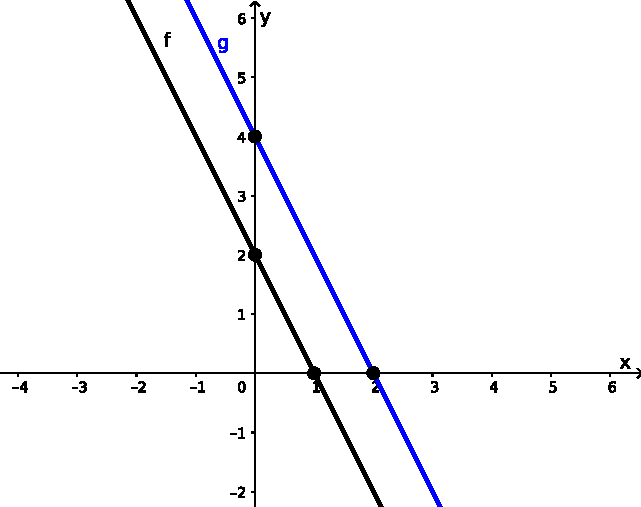
\includegraphics[width=7cm,height=6cm]{./cap_funcao/figs/retasparalelas}}}
   \fbox{\subfigure[Retas perpendiculares]{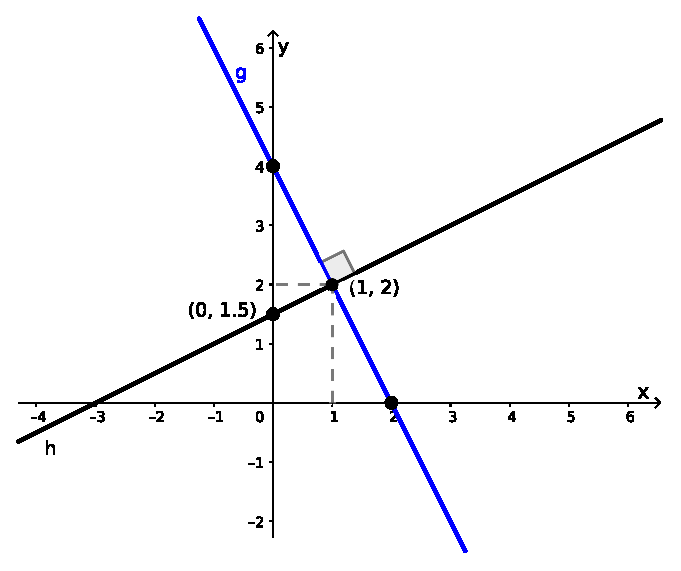
\includegraphics[width=7cm,height=6cm]{./cap_funcao/figs/retasperpendiculares}}}
  \end{figure}
  \end{exem}


 \subsection{Zeros ou raízes das funções afins}

%  \begin{obs}
%  Os zeros ou raízes de uma função $y= f(x)$ são os $x \in Dom(f)$ tais que $f(x)= 0$.
% \end{obs}

 Os zeros de uma função de 1º grau são as raízes da equação $ax+b=0$. Como esta equação é do 1º grau, ela possui uma única raiz, logo a função de 1º grau também possui uma única raiz, que denotaremos por $x'$. Note que o ponto $(x', 0)$ é o ponto de interseção do gráfico da $f$ com o eixo $x$, assim podemos interpretar graficamente as raízes da nossa função como sendo os pontos de interseção do gráfico da função com o eixo das abscissas.

\section{Função (De)crescente}

\begin{obs}
  Sejam $A, B \subset \R$ e uma função real $f: A \rightarrow B$.

  Dizemos que $f$ é uma \textbf{função crescente} em um intervalo $I \subset A$ se, para todo $x, y \in I$,
\begin{equation*}
 x < y \Rightarrow f(x) < f(y).
\end{equation*}

  Dizemos que $f$ é uma \textbf{função decrescente} em um intervalo $I \subset A$ se, para todo $x, y \in I$,
\begin{equation*}
x < y \Rightarrow f(x) > f(y).
\end{equation*}

  Dizemos que $f$ é uma \textbf{função constante} em um intervalo $I \subset A$ se, para todo $x, y \in I$,
\begin{equation*}
x \neq y \Rightarrow f(x) = f(y).
\end{equation*}
\end{obs}

 Seja $f: \R \to \R$ uma função linear dada por $f(x)= ax + b$.

\begin{itemize}
    \item Se \destaque{a > 0} então dados $x_1 < x_2$, temos que:
\begin{equation*}
x_1 < x_2 \Rightarrow ax_1 < ax_2 \Rightarrow ax_1 + b < ax_2 + b \ ,
\end{equation*}
  portanto $f(x_1) < f(x_2)$, neste caso dizemos que $f$ é \textbf{crescente}.

 \item Se \destaque{a < 0} então  dados $x_1 < x_2 \in dom(f)$, temos que:
\begin{equation*}
x_1 < x_2 \Rightarrow ax_1 > ax_2 \Rightarrow ax_1 + b > ax_2 + b \ ,
\end{equation*}
 portanto $f(x_1) > f(x_2)$, neste caso dizemos que $f$ é \textbf{decrescente}.
 \end{itemize}

 Observe que no caso das funções de 1º grau a propriedade de ser crescente ou decrescente é válida em todo o domínio da função, nestes casos dizemos que é uma propriedade global da função.

 \begin{exem}
 Vamos retomar alguns dos nossos exemplos de funções para classificar como crescente, decrescente e constante. Para isso considere $x_1= -2$ e $x_2= 1$, neste caso, $x_1 < x_2$.
  \begin{enumerate}[a)]
   \item Sendo $f(x)= \frac{1}{2}x + 1,5$, temos que
\begin{equation*}
f(x_1)= f(-2)= \frac{1}{2}\cdot (-2) + 1,5= -1 + 1,5= 0,5
\end{equation*}
\begin{equation*}
f(x_2)= f(1)= \frac{1}{2} \cdot 1+\frac{3}{2}= \frac{4}{2}= 2
\end{equation*}
   logo $f(x_1)= 0,5 < 2= f(x_2)$. Portanto $f$ é crescente.
   \item Sendo $f(x)= -2x + 2$, temos que
\begin{equation*}
f(x_1)= f(-2)= -2 \cdot (-2) + 2= 4 + 2= 6
\end{equation*}
\begin{equation*}
f(x_2)= f(1)= -2 \cdot 1 + 2= 0
\end{equation*}
   logo $f(x_1)= 6 > 0 = f(x_2)$. Portanto $f$ é decrescente.
   \item Sendo $f(x)= 2$, temos que
\begin{equation*}
f(x_1)= f(-2)= 2
\end{equation*}
\begin{equation*}
f(x_2)= f(1)= 2
\end{equation*}
   logo $f(x_1)= 2 = 2= f(x_2)$. Portanto $f$ é constante.
  \end{enumerate}
  Como já mostramos acima que para as funções lineares esta propriedade é global, para fazer esta classificação é suficiente testar dois valores de $x$ como fizemos acima.

 \end{exem}

\begin{secExercicios}
    \begin{exer}
        Dada a função $f:\R\to\R$ com $f(x)=x^2-3x+1$, determine:
        \begin{enumerate}[a)]
            \begin{multicols}{3}
                \item $f(-2)$
                \item $f(\sqrt{2})$
                \item $f\left(-\frac{1}{2}\right)$
            \end{multicols}
        \end{enumerate}
    \end{exer}

    \begin{exer}
        Dado o conjunto $A=\{-2,-1,0,1,2\}$, determine a imagem da função $f:A\to\R$ para cada uma das seguintes expressões:
        \begin{enumerate}[a)]
            \item $f(x)=2x$
            \item $f(x)=x^2-1$
            \item $f(x)=x^3$
        \end{enumerate}
    \end{exer}

    \begin{exer}
        Considere as funções $f(x)=-5x+2$ e $g(x)=\frac{2}{3}x+a$. Calcule o valor de $a$ de modo que $f(1)-g(1)=\frac{7}{2}$.
    \end{exer}

    \begin{exer}
        Determine o maoir domínio de cada uma das seguintes funções reais:
        \begin{enumerate}[a)]
            \item $f(x)=4x+5$
            \item $f(x)=\dfrac{1}{-3x+12}$
            \item $f(x)=\sqrt{x+9}$
            \item $f(x)=\sqrt{x-1}+\sqrt{1-x}$
            \item $f(x)=\dfrac{x}{x^2-x-6}+\dfrac{1}{x+4}$
            \item $f(x)= \dfrac{1}{\sqrt[3]{x}}$
            \item $f(x)=\sqrt{x-2}+\dfrac{x+1}{x-3}$
            \item $f(x)=\dfrac{x+1}{\sqrt{x^2-4}}$
            \item $f(x)=\dfrac{\sqrt{x+1}}{x^3} + \dfrac{2x}{\sqrt{x+4}}$
        \end{enumerate}
    \end{exer}
    
    \begin{exer}
        Dada a função $f(x)=-x^2+2x$, simplifique:
        \begin{enumerate}[a)]
        \begin{multicols}{2}
            \item $\dfrac{f(x)-f(1)}{x-1}$
            \item $\dfrac{f(x+h)-f(x)}{h}$
        \end{multicols}
        \end{enumerate}
    \end{exer}

    \begin{exer}
        Simplifique $\frac{f(x)-f(p)}{x-p}$, com $x\neq p$, para cada uma das funções a seguir:
        \begin{enumerate}[a)]
            \item $f(x)=2x+1$ para $p=0$.
            \item $f(x)=x^2$ para $p=1$.
            \item $f(x)=x^3$ para $p=2$.
            \item $f(x)=\frac{1}{x}$ para $p=1$.
            \item $f(x)=-x+4$ para $p$ qualquer.
            \item $f(x)=x^2$ para $p$ qualquer.
        \end{enumerate}
    \end{exer}

    \begin{exer}
        Determine o maior domínio, imagem e esboce o gráfico de cada umas das funções a seguir:
        \begin{enumerate}[a)]
        \begin{multicols}{2}
            \item $f(x)=\frac{5}{4}$
            \item $f(x)=-3x$
            \item $f(x)=2x-6$
            \item $f(x)=\frac{1}{2}x +2$
        \end{multicols}
        \end{enumerate}
    \end{exer}

    \begin{exer}
        Estude o sinal das seguintes funções:
        \begin{enumerate}[a)]
            \item $f(x)=4x-5$
            \item $f(x)=2-3x$
            \item $f(x)=\frac{x}{3}-1$
            \item $f(x)=2x+5$
            \item $f(x)=-5x+1$
        \end{enumerate}
    \end{exer}

    \begin{exer}
        Considere as funções reais dadas por $f(x)=8-x$ e $g(x)=3x$. Calcule o ponto de interseção do gráfico detas funções.
    \end{exer}

    \begin{exer}
        Seja $f$ uma função afim tal que $f(3)=5$ e $f(-2)=-5$. Calcule $f\left(\frac{1}{2}\right)$.
    \end{exer}

    \begin{exer}
        Considere a função real $f(x)$ tal que $f(1)=43$ e $f(x+1)=2f(x)-15$. Determine o valor de $f(0)$.
    \end{exer}

    \begin{exer} Determine a expressão de cada uma das funções para cada um dos gráficos abaixo
        \begin{enumerate}[a)]
            \item 
            \begin{tikzpicture}[scale=0.7]
            \tkzInit[xmin=-3, xmax=3, xstep=1, ymin=-1,ymax=4]
                %\tkzDrawXY
                \tkzAxeXY
                
                \tkzFct[thick,red]{2*x+3}
            
                %\tkzDefPointByFct[ref=A, with=a](-1)
                \tkzDefPoint(-1,1){A}
                \tkzDefPoint(0,3){B}
                \tkzPointShowCoord(A)
                \tkzDrawPoint[fill=red, size=3](A)
                \tkzDrawPoint[fill=red, size=3](B)
                
            \end{tikzpicture}

            \item 
            \begin{tikzpicture}[scale=0.7]
            \tkzInit[xmin=-3, xmax=3, xstep=1, ymin=-1,ymax=3]
                %\tkzDrawXY
                \tkzAxeXY
                
                \tkzFct[thick,red]{-0.5*x+1}
            
                %\tkzDefPointByFct[ref=A, with=a](-1)
                \tkzDefPoint(0,1){A}
                \tkzDefPoint(2,0){B}
                %\tkzPointShowCoord(A)
                \tkzDrawPoint[fill=red, size=3](A)
                \tkzDrawPoint[fill=red, size=3](B)
                
            \end{tikzpicture}

            \item 
            \begin{tikzpicture}[scale=0.7]
            \tkzInit[xmin=-3, xmax=3, xstep=1, ymin=-2,ymax=1]
                %\tkzDrawXY
                \tkzAxeXY
                
                \tkzFct[thick,red]{0.666*x-1}
            
                %\tkzDefPointByFct[ref=A, with=a](-1)
                \tkzDefPoint(3,1){A}
                \tkzDefPoint(0,-1){B}
                \tkzPointShowCoord(A)
                \tkzDrawPoint[fill=red, size=3](A)
                \tkzDrawPoint[fill=red, size=3](B)
                
            \end{tikzpicture}

            \item 
            \begin{tikzpicture}[scale=0.7]
            \tkzInit[xmin=-2, xmax=4, xstep=1, ymin=-4,ymax=1]
                %\tkzDrawXY
                \tkzAxeXY
                
                \tkzFct[thick,red]{-0.75*x}
            
                %\tkzDefPointByFct[ref=A, with=a](-1)
                \tkzDefPoint(4,-3){A}
                \tkzDefPoint(0,0){B}
                \tkzPointShowCoord(A)
                \tkzDrawPoint[fill=red, size=3](A)
                \tkzDrawPoint[fill=red, size=3](B)
            \end{tikzpicture}
        \end{enumerate}
    \end{exer}

    \begin{exer}
        Seja $f(2x+7)=-4x+9$. Determine o valor de $f(-5)$.
    \end{exer}

    \begin{exer}
        Determine os possíveis valores de $p$ para que a função $f(x)=(2p+3)x+2$ seja decrescente.
    \end{exer}

    \begin{exer}
        Determine o valor de $p$ de modo que o gráfico da função $f(x)=2x+p+3$ passe pelo ponto $(1,2)$.
    \end{exer}
    
    \begin{exer}
        Dadas as funções $f$ e $g$ cujas expressões são $f(x)=ax+4$ e $g(x)=bx+1$, calcule $a$ e $b$ de modo que os gráficos das funções interseptem-se no ponto $(1,6)$.
    \end{exer}
    
    \begin{exer}
 Uma bolsa de valores tinha um preço de R\$ $42,00$ quando sofreu uma queda de R\$$2,50$ por dia, durante $5$ dias seguidos.
  \begin{enumerate}[a)]
  \item Qual é a função que representa a queda do valor dessa ação em função do dia?
  \item Represente, no plano cartesiano, os pontos correspondentes a esses $5$ dias e o segmento de reta que passa por esses pontos.
  \end{enumerate}
  \end{exer}
  \begin{resp}
    a) $f(x)= 42 - 2,50 x$; b) a cargo do leitor;
  \end{resp}
  
  \begin{exer}
  Um táxi, realizando uma corrida, cobra uma taxa fixa denominada bandeira de R\$$3,50$ e R\$$0,80$ por quilômetro rodado.
  Com base nesses dados, determine:
  \begin{enumerate}[a)]
  \item A função que representa o valor pago por uma corrida de $x$ quilômetros.
  \item Quantos quilômetros foram rodados se a conta foi de R\$ $17,10$.
  \end{enumerate}
  \end{exer}
  \begin{resp}
    a) $f(x)= 3,50 + 0,80 x$; b) $x= 17 Km$;
  \end{resp}
  
  \begin{exer}
  Para cercar um terreno, tem-se duas opções:
  1ª) Taxa de entrega no local R\$ $100,00$ e R\$$12,00$ o metro linear de cerca.
  2ª) Taxa de entrega no local R\$ $80,00$ e R\$ $15,00$ o metro linear de cerca.
  \begin{enumerate}[a)]
  \item Represente o custo de cada opção para $x$ metros de cerca.
  \item Qual das duas opções é mais vantajosa para $140$m de perímetro.
  \end{enumerate}
  \end{exer}
  \begin{resp}
    a) 1ª opção: $f(x)= 100 + 12x$, 2ª opção: $f(x)= 80+15x$; b) 1ª opção; 
  \end{resp}
  
%   \begin{exer}
%   No Brasil, o sistema de numeração de sapatos ou tênis é baseado na fórmula $N(p)= \frac{5p + 28}{4}$, que indica o valor aproximado do número do calçado $N$ em função do comprimento $p$, em centímetros do pé da pessoa. Determine o número do sapato ou tênis que uma pessoa deve comprar se, ao medir o comprimento de seu pé obteve:
%   \begin{enumerate}[a)]
%   \item $22,8$ cm
%   \item $24$ cm
%   \item $26,4$ cm
%   \end{enumerate}
%   \end{exer}
%   \begin{resp}
%     a) $35,5$; b) $37$; c) $40$;
% %    \par\noindent\rule{\columnwidth}{0.4pt}
%   \end{resp}
\end{secExercicios}

%\subsection*{Respostas}

%\shipoutAnswer

 




%\subsection*{Respostas}

%\shipoutAnswer



%\subsection*{Respostas}

%\shipoutAnswer

 